\section{Introduction}
\label{sec:layeredbsdf:intro}

Physically-based shading models have become mature and commonplace in recent years across a number of rendering applications, within entertainment, architecture, and industrial design. 
However, we are seeing constant progress in the area of material reflection and scattering models, aiming to achieve higher physical realism and to enable more effective material content creation.

Many real world materials are comprised of thin layers with varying compositions. For example, metallic paint is a dielectric coating covering a metallic substrate composed of randomly oriented aluminum flakes; the absorption and scattering properties of the dielectric layer give the material its color and modify its directional scattering properties as well.
Many biological materials (e.g. plant leaves) are also layered, and their appearance is a complex combination of the absorption properties, scattering phase function, air-material interface roughness, and thickness variation.
Different characteristics of such interfaces and volumetric scattering properties can produce richly diverse material appearances from anisotropic highlights to complex textures. Furthermore, detailed layer thickness variations, scratches and bumps on the layer interfaces give these materials additional richness. Accurately understanding and simulating these interactions is therefore key to further progress in the rendering of materials.

\begin{figure}[h]
	\centering
	\setlength{\resLen}{2.in}
	\addtolength{\tabcolsep}{-3pt}
	\begin{tabular}{ccccc}
		\begin{overpic}[height=\resLen]{layeredbsdf/teaser/teaser.jpg}
			\put(2,3){\color{white} \textbf{(a)}}
		\end{overpic}
		&
		\begin{overpic}[height=\resLen]{layeredbsdf/teaser/green.jpg}
			\put(2,3){\color{white} \textbf{(b1)}}
		\end{overpic}
		&
		\begin{overpic}[height=\resLen]{layeredbsdf/teaser/yellow.jpg}
			\put(2,3){\color{white} \textbf{(c1)}}
		\end{overpic}
		&
		\begin{overpic}[height=\resLen]{layeredbsdf/teaser/blue.jpg}
			\put(2,3){\color{white} \textbf{(d1)}}
		\end{overpic}
		&
		\begin{overpic}[height=\resLen]{layeredbsdf/teaser/magenta.jpg}
			\put(2,3){\color{white} \textbf{(e1)}}
		\end{overpic}
	\end{tabular}
	\\[2pt]
	\setlength{\resLen}{2.8in}
	\addtolength{\tabcolsep}{4pt}
	\begin{tabular}{cc}
		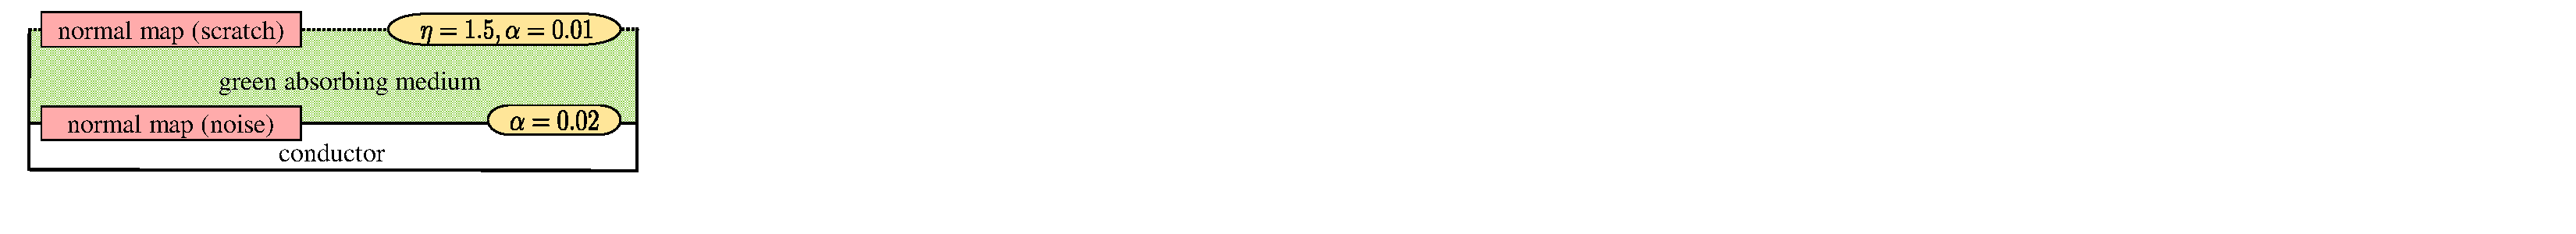
\includegraphics[width=\resLen]{layeredbsdf/teaser/green.pdf} &
		
\includegraphics[width=\resLen]{layeredbsdf/teaser/yellow.pdf} \\
		\textbf{(b2)} & \textbf{(c2)} \\
		
\includegraphics[width=\resLen]{layeredbsdf/teaser/blue.pdf} &
		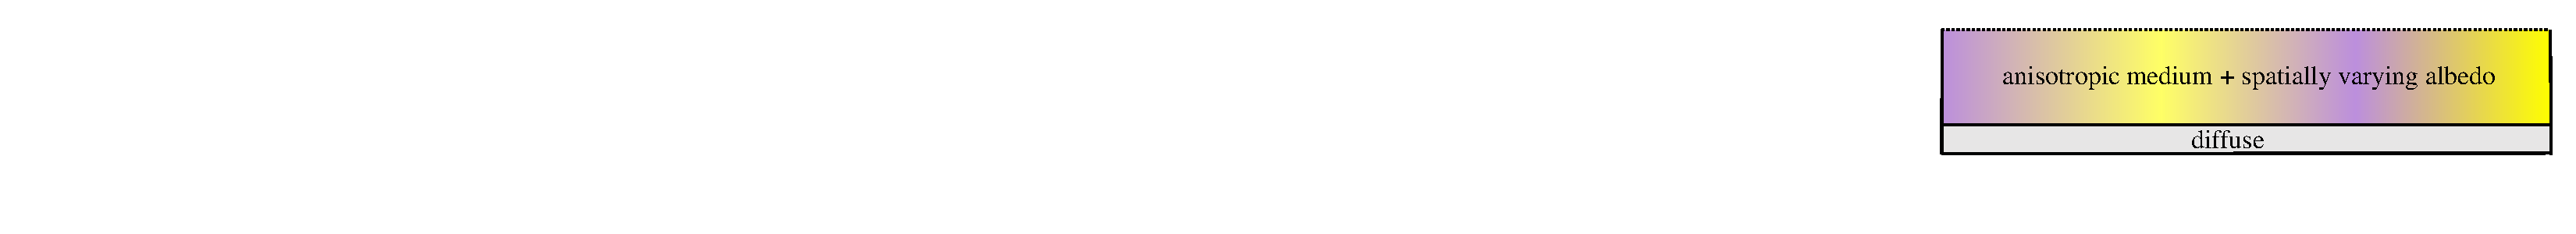
\includegraphics[width=\resLen]{layeredbsdf/teaser/magenta.pdf} \\
		\textbf{(d2)} & \textbf{(e2)}
	\end{tabular}
	\caption[Teaser of LayeredBSDF]{\label{fig:layeredbsdf:teaser}
		We introduce a new BSDF model leveraging an efficient Monte Carlo simulation algorithm applied locally to layered geometries.
		Our model enjoys the flexibility of using arbitrary layer interfaces and internal media and is capable of reproducing a wide variety of appearances.
		This example contains three vases on a tablecloth, all described using our BSDF model (see the insets for layer configurations).
	}
\end{figure}


However, explicitly simulating light-layer interactions by modeling the full geometry of these layers would be very expensive and cumbersome. 
The complex and spatially varying interface and internal microgeometries are much too costly to describe and simulate using standard 3D scene modeling tools such as triangle meshes and volumetric grids.
Furthermore, due to the presence of multiple refractive interfaces, it can be very challenging to correctly construct light transport paths that connect light scattering locations to light sources, a key operation in most practical Monte Carlo rendering systems. Cheap approximations to these light transport problems (e.g. ignoring refraction, or composing layers using simple blending) are not sufficient to achieve true realism.

A few techniques have been developed to address this problem. Weidlich and Wilkie \cite{weidlich2007arbitrarily} construct a simple and flexible analytical model. However, significant approximations are necessary; interface roughness is not fully handled for transmission, and no volumetric scattering is supported. The work of Belcour \cite{belcour2018efficient} recently introduced a more advanced approach based on tracking low-order moments of the BSDF lobes; however, it still introduces some approximations and limitations. On the other hand, Jakob et al. \cite{jakob2014comprehensive} (with a recent follow-up \cite{zeltner2018layer}) introduce a solution that is very accurate, but expensive: it represents BSDFs as discretized datasets and relies on expensive Fourier-domain operations on these to implement layer composition and thickness adjustment. This makes free spatial variation of the layer properties prohibitively expensive: a significant limitation in practice.

In this paper, we introduce a new layered BSDF model without the above limitations. Our model provides an accurate, unbiased solution; to our knowledge, it is the only such model.
Unlike previous work, we do not attempt to derive an analytic model for the BSDF lobe shapes. Instead, inside the evaluation and sampling routines of the layered BSDF, we run a Monte Carlo simulation of light transport within flat slabs.
This is substantially faster than explicitly constructing the layer geometry, because no expensive scene ray tracing is required.
Our model computes an accurate solution of the layered light transport problem.
It is based on physical interface and volume scattering models, conserves energy and is reciprocal when possible. It can also be easily integrated into standard Monte Carlo rendering systems.
This requires no precomputation and thus can efficiently handle spatially varying appearances. It also supports the full range of editability of the layer properties, both interface and volumetric, and allows anisotropy in both interface BSDFs and phase functions. In fact, the only limiting assumption of our model is the layer assumption itself.

Our solution is fundamentally more powerful at constructing light transport paths than generic transport algorithms (e.g standard path tracing, bidirectional or Metropolis transport); see Figure \ref{fig:layeredbsdf:equal_time_compare}. We introduce a modified path integral framework for light transport in flat slabs, superior to the standard path formulation in this setting. Because it is based on a product of solid angle instead of area measures, it does not contain the high-variance geometry terms needed in standard algorithms. We introduce two simulation techniques within this formulation: the first is analogous to a forward path tracer with next event estimation through layer boundaries and multiple importance sampling; the second is a fully bidirectional estimator. We show the capabilities of this solution on a number of examples, featuring multiple layers with surface and volumetric scattering. Our examples show spatial variation in all parameters: surface BSDF, volume and phase function parameters, layer thickness and surface normal. See Figure \ref{fig:layeredbsdf:teaser}.

